\documentclass[12pt]{article}
\usepackage[T1]{fontenc}
%\usepackage[latin9]{inputenc}
\usepackage[utf8]{inputenc}
\usepackage[english]{babel}
\usepackage{amsmath}
\usepackage{amsfonts}
\usepackage{amssymb}
\usepackage{setspace}
\usepackage{rotating}
\usepackage{graphics}
\usepackage[round]{natbib}
%\usepackage{graphicx}
%\usepackage{float} 				%allows you to float images
\usepackage{latexsym}
\usepackage{bbding}
%\usepackage {moresize}
\usepackage{listings}
\usepackage{bbding}
\usepackage{blindtext}
\usepackage{hhline}
%\usepackage{tikz}
%\usetikzlibrary{shapes,backgrounds}
%\usepackage{pgfplots}
%\usetikzlibrary{arrows}
\usepackage{enumitem}
\doublespacing
%\usepackage{geometry}
\usepackage{amsthm}
\usepackage{color}
%\usepackage{array,multirow}
%\usepackage{subcaption}
%\usepackage{pst-plot}
%	\psset{xunit=15mm}
%\geometry{verbose,tmargin=1in,bmargin=1in,lmargin=.5in,rmargin=.5in}
\setlength{\parskip}{\bigskipamount}
\setlength{\parindent}{0pt}
\usepackage{multicol}

\newenvironment{problem}[3][Problem]{\begin{trivlist}
\item[\hskip \labelsep {\bfseries #1}\hskip \labelsep {\bfseries #2.}]}{\end{trivlist}}

\title{Problem Set 2 \thanks{Problems 1,2,3,4,5,6}}
\author{Ian McGroarty \\
	Course Number: 625.641}
\date{June 18, 2019}

\begin{document}

\maketitle
\section{Definitions}
\underline{Def: Forward Rate Formulas} (pg 79). The implied forward rate between times $t_1$ and $t_2$ is the rate of interset between those times that is consistent with a given spot rate curve. For Yearly compounding, the forward rate is:  
\begin{align*}
f_{i,j} =& [\frac{(1+s_j)^j}{(1+s_i)^i}]^{1/(j-i)}-1 \\
 e^{s(t_2)t_2} =& e^{s(t_1)t_1}e^{f_{t_1,t_2}(t_2-t_1)}
\end{align*}

\underline{Discount Factor Relation} The discount facot between periods i and j is defined as $$ d_{i,j}=[\frac{1}{1+f_{i,j}}]^{j-i}$$ These factors satisfy the compounding rule: $d_{i,k}=d_{i,j}d_{j,k}$\\

\underline{Def. Derivative (Ross pg 223)} Let F be a real valued function defined on an open interval contained a point a. We say f is differentiable at a, or f has derivative at a if the limit $$ f'(a) = \lim_{x \to a} \frac{f(x)-f(a)}{x-a} $$

\newpage
%%%%%%%%%%%%%%%%%%%%%%%%%%%%%%%%%%%%%%%%%%%%%%%%%%%%%%%%
%%%%%%%%%%%%%%%%%%%%%%%%%%%%%%%%%%%%%%%%%%%%%%%%%%%%%%%%%%%%%%%%%%%%%%%%%%%%%%%%%%%%%%%%%%%%%%%%%%%%%%%%%%%%%%%%
%%%%%%%%%%%%%%%%%%%%%%%%%%%%%%%%%%%%%%%%%%%%%%%%%%%%%%%%%%%%%%%%%%%%%%%%%%%%%%%%%%%%%%%%%%%%%%%%%%%%%%%%%%%%%%%%
\begin{problem}1. If spot rates for 1 and 2 years are $s_1 = 6.3\%$ and $s_2 = 6.9\%$ what is the forward rate $f_{1,2}$ \\
\textbf{Solution} Using the definition above: 
\begin{align*}
 f_{i,j} &= [\frac{(1+s_j)^j}{(1+s_i)^i}]^{1/(j-i)}-1 && \text{Def. Forward Rate (pg 79)} \\ 
&= [\frac{(1+s_2)^2}{(1+s_1)^1}]^{1/(2-1)}-1 \\ 
&= [\frac{(1+6.9)^2}{(1+6.3)}]-1 \\
f_{1,2} &= 7.5493 \%
\end{align*}
\end{problem}
%%%%%%%%%%%%%%%%%%%%%%%%%%%%%%%%%%%%%%%%%%%%%%%%%%%%%%%%
%%%%%%%%%%%%%%%%%%%%%%%%%%%%%%%%%%%%%%%%%%%%%%%%%%%%%%%%

\begin{problem}2. Given the (yearly) spot rate curve $s=(5.0,5.3,5.6,5.8,6.0,6.1)$ find the spot rate curve for next year. \\
\textbf{Solution} The forcast spot rate is found using:
$$ s`_{j-1}= f_{1,j}=[\frac{(1-s_j)^j}{1+s_1}]^{1/(j-1)}-1 $$
This gives us a forcasted  $s_7 = 6.34$\\

\begin{tabular}{l|cccccc}
                 & s1  & s2     & s3    & s4     & s5    & s6 \\ 
\hline
  Current  & 5.0 & 5.3   & 5.6   & 5.8   & 6.0   & 6.1 \\
  Forecast  &     &  5.62 & 5.92 & 6.09 & 6.28 & 6.34  \\
\end{tabular}
\end{problem}
%%%%%%%%%%%%%%%%%%%%%%%%%%%%%%%%%%%%%%%%%%%%%%%%%%%%%%%%
%%%%%%%%%%%%%%%%%%%%%%%%%%%%%%%%%%%%%%%%%%%%%%%%%%%%%%%%

\begin{problem}3. Consider two 5-year bonds: one has 9\% coupon and sells for 101.00; the other has a 7\% coupon and sells for 93.30 Find the price of a 5-year (zero?) coupon bond. (This question is confusing but I'm assuming it is following the structure of Example 4.3)  \\
\textbf{Solution} To construct a zero coupon bond we first must make the sum of the coupons equal zero: Let $x_A$ represent the amount of the 9\% coupon bond and $x_B$ represent the amount of the 7\% coupon bond held. 
$$ 0.09x_A + 0.07x_B $$
We also want the year 5 payout to be 100 to match the face value of 100 of a zero coupon bond. 
$$ 109x_A + 107x_B $$
We can solve these equations for $x_A=-3.5$ and $x_B=4.5$. To evaluate the price of the constructed zero coupon bond: 
$$ P_Ax_A + P_Bx_B = (101)*(-3.5) + (93.2)*(4.5) = 65.9 $$

\end{problem}

%%%%%%%%%%%%%%%%%%%%%%%%%%%%%%%%%%%%%%%%%%%%%%%%%%%%%%%%
%%%%%%%%%%%%%%%%%%%%%%%%%%%%%%%%%%%%%%%%%%%%%%%%%%%%%%%%
\begin{problem}5. Let $s(t), 0 \leq t \leq \infty$, denote a spot rate curve; that is the present value of a dollar to be recieved at time t is $e^{-s(t)t}$. For $t_1 < t_2$ let $f(t_1,t_2)$ be the forward rate between $t_1$ and $t_2$ implied by the spot rate curve.\\
\textbf{(a)}. Find an expression for $f_{t_1,t_2}$\\
\textbf{(b)}. Let $r(t) = \lim_{t_2\to t} f(t_1,t_2)$ . We can call $r(t)$ the \underline{instantaneuous interest rate} at time t. Show that $r(t) = s(t) + s'(t)t$ \\
\textbf{(c)} $x_0$ is invested at $t=0$ with instantaneous rate of interest $r(t)$ at all t (compounded). Then x(t) will satisfy $dx(t)/d=r(t)x(t)$. Find x(t). 

\textbf{Solution} 
\begin{align*}
e^{s(t_2)t_2} =& e^{s(t_1)t_1}e^{f_{t_1,t_2}(t_2-t_1)} && \text{Forward Rate Formula c (pg 79)} \\
s(t_2)t_2 =& s(t_1)t_1 + f_{t_1,t_2}(t_2-t_1) && \text{take the log} \\
f_{t_1,t_2} =& \frac{s(t_2)t_2 -s(t_1)t_1}{(t_2-t_1)}  && \text{solve for f} \\
\hline \\
\lim_{t_2 \to t} f_{t,t_2} =& \frac{s(t_2)t_2 -s(t)t}{(t_2-t)}  \\
r(t)=& \frac{d}{dt}[s(t)t] && \text{Def. Derivative} \\
r(t)=& s(t) + s'(t)t && \text{product rule} \\
\hline
\frac{d}{dt}x(t) =&r(t)x(t) \\
\frac{d}{dt}x(t) =& x(t) \cdot\frac{d}{dt}[s(t)t] && \text{Substitute r(t)} \\
\frac{d}{dt}x(t) \cdot \frac{1}{x(t)} =&  \frac{d}{dt}[s(t)t] \\ 
\frac{d}{dt}ln(x(t)) =&  \frac{d}{dt}[s(t)t] && \text{Note: chain rule ln(x(t))} \\
ln(x(t)) =& s(t)t && \text{Integrate} \\
x(t) =& e^{s(t)t} 
\end{align*}


\end{problem}

%%%%%%%%%%%%%%%%%%%%%%%%%%%%%%%%%%%%%%%%%%%%%%%%%%%%%%%%
%%%%%%%%%%%%%%%%%%%%%%%%%%%%%%%%%%%%%%%%%%%%%%%%%%%%%%%%

%%%%%%%%%%%%%%%%%%%%%%%%%%%%%%%%%%%%%%%%%%%%%%%%%%%%%%%%
%%%%%%%%%%%%%%%%%%%%%%%%%%%%%%%%%%%%%%%%%%%%%%%%%%%%%%%%

\begin{problem}6. At time zero the one period discount rates are shown in column 1 and 2 below: Fine the time zero discount factors as shown in column 3 and 4 below. \\

\textbf{Solution}  We can use the compounding rule here to find $d_{0,2}=d_{0,1}d_{1,2} \cdots d_{0,6}=d_{0,1}...d_{5,6}$ I preformed these calculations in an excel table and the result is shown below. 
\begin{center}
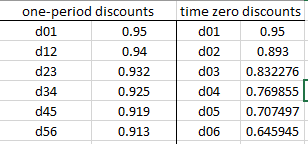
\includegraphics[width=0.59\linewidth]{mod3p3.png}
\end{center}

%$d_{0,1},d_{1,2},d_{2,3},d_{3,4},d_{4,5},d_{5,6} $
\end{problem}
\end{document}

https://www.investopedia.com/university/advancedbond/bond-pricing.asp
https://quant.stackexchange.com/questions/22288/duration-of-perpetual-bond
http://people.stern.nyu.edu/gyang/foundations/sample-final-solutions.html
http://pages.stern.nyu.edu/~jcarpen0/courses/b403333/07convexh.pdf
https://web.stanford.edu/class/msande247s/2009/summer%2009%20week%205/Bond%20Formula%20Sheet.pdf


\underline{Def: Forward Rate Formulas} (pg 79). The implied forward rate between times $t_1$ and $t_2$ is the rate of interset between those times that is consistent with a given spot rate curve. For Yearly compounding, the forward rate is:  
\begin{align*}
f_{i,j} =& [\frac{(1+s_j)^j}{(1+s_i)^i}]^{1/(j-i)}-1 \\
 e^{s(t_2)t_2} =& e^{s(t_1)t_1}e^{f_{t_1,t_2}(t_2-t_1)}
\end{align*}

\underline{Discount Factor Relation} The discount facot between periods i and j is defined as $$ d_{i,j}=[\frac{1}{1+f_{i,j}}]^{j-i}$$ These factors satisfy the compounding rule: $d_{i,k}=d_{i,j}d_{j,k}$\\

\underline{Def. Derivative (Ross pg 223)} Let F be a real valued function defined on an open interval contained a point a. We say f is differentiable at a, or f has derivative at a if the limit $$ f'(a) = \lim_{x \to a} \frac{f(x)-f(a)}{x-a} $$
